\documentclass[12pt]{article}
\usepackage{amsfonts, amssymb, amsmath, amsthm}
\usepackage[margin=1in]{geometry}
\usepackage{tikz}
\usetikzlibrary{patterns, decorations.pathreplacing}

\pagestyle{myheadings}
\markright{Explainer: Rudin 1.5 — Infimum and Supremum Duality\hfill}

\newcommand{\R}{\mathbb{R}}
\newcommand{\Q}{\mathbb{Q}}

\begin{document}

\begin{center}
    \textbf{\Large Infimum and Supremum Duality}\\[0.5em]
    \large A visual guide to Rudin 1.5
\end{center}

\section{The Claim}

If $A \subseteq \mathbb{R}$ is nonempty and bounded below, and $-A = \{-x : x \in A\}$, then:
\[
\inf A = -\sup(-A)
\]

\section{What is $-A$?}

$-A$ is the set $A$ ``reflected'' across zero.

\begin{center}
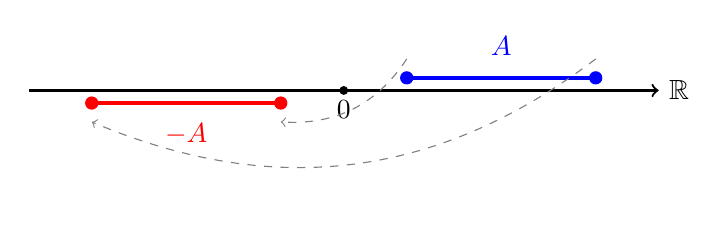
\begin{tikzpicture}[scale=0.8]
    \draw[thick, ->] (-5, 0) -- (5, 0) node[right] {$\mathbb{R}$};

    % A
    \draw[blue, ultra thick] (1, 0.2) -- (4, 0.2);
    \fill[blue] (1, 0.2) circle (3pt);
    \fill[blue] (4, 0.2) circle (3pt);
    \node[blue] at (2.5, 0.7) {$A$};

    % -A
    \draw[red, ultra thick] (-4, -0.2) -- (-1, -0.2);
    \fill[red] (-4, -0.2) circle (3pt);
    \fill[red] (-1, -0.2) circle (3pt);
    \node[red] at (-2.5, -0.7) {$-A$};

    % Zero
    \fill (0, 0) circle (2pt) node[below] {$0$};

    % Reflection arrows
    \draw[dashed, gray, ->] (1, 0.5) to[bend left] (-1, -0.5);
    \draw[dashed, gray, ->] (4, 0.5) to[bend left] (-4, -0.5);
\end{tikzpicture}
\end{center}

\section{The Key Relationship}

\begin{center}
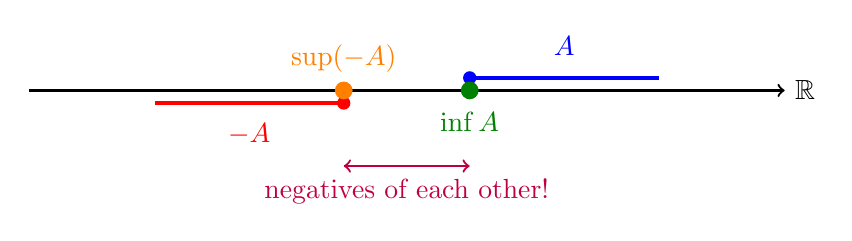
\begin{tikzpicture}[scale=0.8]
    \draw[thick, ->] (-6, 0) -- (6, 0) node[right] {$\mathbb{R}$};

    % A with inf
    \draw[blue, ultra thick] (1, 0.2) -- (4, 0.2);
    \fill[blue] (1, 0.2) circle (3pt);
    \node[blue] at (2.5, 0.7) {$A$};

    % inf A
    \fill[green!50!black] (1, 0) circle (4pt);
    \node[green!50!black] at (1, -0.5) {$\inf A$};

    % -A with sup
    \draw[red, ultra thick] (-4, -0.2) -- (-1, -0.2);
    \fill[red] (-1, -0.2) circle (3pt);
    \node[red] at (-2.5, -0.7) {$-A$};

    % sup(-A)
    \fill[orange] (-1, 0) circle (4pt);
    \node[orange] at (-1, 0.5) {$\sup(-A)$};

    % The relationship
    \draw[<->, thick, purple] (1, -1.2) -- (-1, -1.2);
    \node[purple] at (0, -1.6) {negatives of each other!};
\end{tikzpicture}
\end{center}

\section{Why Does This Work?}

Negation \textbf{reverses inequalities}:
\[
a \leq b \quad \Longleftrightarrow \quad -a \geq -b
\]

So:
\begin{itemize}
    \item Lower bounds of $A$ become upper bounds of $-A$
    \item The \textbf{greatest} lower bound of $A$ becomes the \textbf{least} upper bound of $-A$
\end{itemize}

\section{The Proof in Pictures}

\textbf{Step 1:} $\inf A$ is a lower bound of $A$

\begin{center}
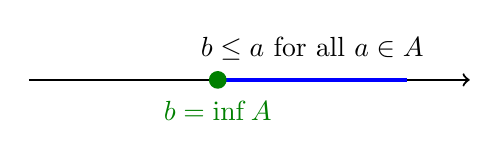
\begin{tikzpicture}[scale=0.8]
    \draw[thick, ->] (-1, 0) -- (6, 0);
    \draw[blue, ultra thick] (2, 0) -- (5, 0);
    \fill[green!50!black] (2, 0) circle (4pt);
    \node[green!50!black] at (2, -0.5) {$b = \inf A$};
    \node at (3.5, 0.5) {$b \leq a$ for all $a \in A$};
\end{tikzpicture}
\end{center}

\textbf{Step 2:} So $-\inf A$ is an upper bound of $-A$

\begin{center}
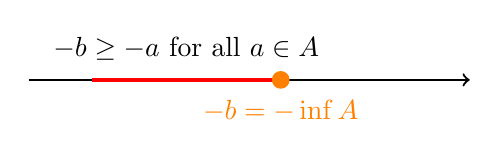
\begin{tikzpicture}[scale=0.8]
    \draw[thick, ->] (-6, 0) -- (1, 0);
    \draw[red, ultra thick] (-5, 0) -- (-2, 0);
    \fill[orange] (-2, 0) circle (4pt);
    \node[orange] at (-2, -0.5) {$-b = -\inf A$};
    \node at (-3.5, 0.5) {$-b \geq -a$ for all $a \in A$};
\end{tikzpicture}
\end{center}

\textbf{Step 3:} $-\inf A$ is the \textbf{least} upper bound of $-A$

Why? If $c$ is any upper bound of $-A$, then $-c$ is a lower bound of $A$. Since $\inf A$ is the greatest lower bound: $-c \leq \inf A$, so $c \geq -\inf A$.

\section{Summary}

\begin{center}
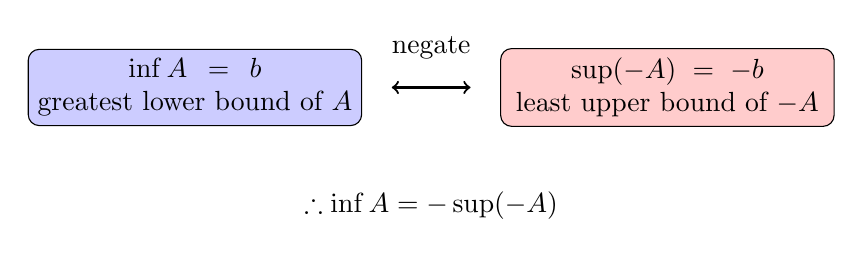
\begin{tikzpicture}
    \node[draw, rounded corners, fill=blue!20, text width=4cm, align=center] at (-3, 0) {
        $\inf A = b$\\
        greatest lower bound of $A$
    };

    \node[draw, rounded corners, fill=red!20, text width=4cm, align=center] at (3, 0) {
        $\sup(-A) = -b$\\
        least upper bound of $-A$
    };

    \draw[<->, thick] (-0.5, 0) -- (0.5, 0);
    \node at (0, 0.5) {negate};

    \node at (0, -1.5) {$\therefore \inf A = -\sup(-A)$};
\end{tikzpicture}
\end{center}

\section{Intuition}

Think of it as a mirror:
\begin{itemize}
    \item The infimum of $A$ is on the ``left edge'' of $A$
    \item When you reflect across zero, left becomes right
    \item So the infimum of $A$ becomes the supremum of $-A$ (negated)
\end{itemize}

\end{document}
